% 
%
% (c) 2025 Autor, ETH Zürich
%
% !TEX root = linalg_I-II_summary.tex
% !TEX encoding = UTF-8
%

\section{Euclidean \& Hermitian (unitary) Spaces}
At last we endow our spaces with a geometric structure. We work here with vector spaces $V$ over $K = \mathbb{R}$ or $K = \mathbb{C}$. Over $\mathbb{R}$ we'll have Euclidean spaces. Over $\mathbb{C}$ we'll have Hermitian (a.k.a unitary) spaces.

\begin{definition}{Scalar Product}{scalar_prod}
	Let $V$ be a vector space over $\mathbb{R}$. A \textbf{scalar product} (a.k.a inner product) is a function $V \times V \to \mathbb{R}, \quad (v, w) \mapsto \langle v, w\rangle$ that has the following properties:
	\begin{enumerate}
		\item Linearity in the first variable:
		\begin{align*}
			\langle v_1 + v_2, w\rangle &= \langle v_1, w\rangle + \langle v_2, w\rangle \qquad \forall \, v_1, v_2, w \in V\\
			\langle \alpha v, w\rangle &= \alpha \, \langle v, w\rangle \qquad \forall\, \alpha \in \mathbb{R}, v, w \in V. 
		\end{align*}
		\item Linearity in the second variable:
		\begin{align*}
			\langle v, w_1, w_2\rangle &= \langle v, w_1\rangle + \langle v, w_2\rangle \qquad \forall \, v, w_1, w_2 \in V\\
			\langle v, \alpha w\rangle &= \alpha \, \langle v, w\rangle \qquad \forall\, \alpha \in \mathbb{R}, v, w \in V. 
		\end{align*}
		\item Symmetry:
		\[
			\langle v, w \rangle = \langle w, v \rangle \qquad \forall \, v, w \in V.
		\]
		\item Positivity:
		\[
			\langle v, v \rangle > 0 \qquad \forall \, v \in V \setminus \{0\}.
		\]
	\end{enumerate}
	
	We call $\big(V, \langle \cdot , \cdot \rangle\big)$ an \textbf{Euclidean space}, or a space endowed with a scalar product.
\end{definition}

\begin{definition}{Hermitian Product}{hermit_prod}
	Let $V$ be a vector space over $\mathbb{C}$. A \textbf{Hermitian product} (or inner product) on $V$ is a function $V \times V \to \mathbb{C}, \quad (v, w) \mapsto \langle v, w \rangle$ with the following properties:
	\begin{enumerate}
		\item Linearity in the first variable:
		\begin{align*}
			\langle v_1 + v_2, w\rangle &= \langle v_1, w\rangle + \langle v_2, w\rangle \qquad \forall \, v_1, v_2, w \in V\\
			\langle \alpha v, w\rangle &= \alpha \, \langle v, w\rangle \qquad \forall\, \alpha \in \mathbb{C}, v, w \in V. 
		\end{align*}
		\item Sesquilinearity (complex anti-linearity) in the second variable:
		\begin{align*}
			\langle v, w_1, w_2\rangle &= \langle v, w_1\rangle + \langle v, w_2\rangle \qquad \forall \, v, w_1, w_2 \in V\\
			\langle v, \alpha w\rangle &= \overline{\alpha} \, \langle v, w\rangle \qquad \forall\, \alpha \in \mathbb{C}, v, w \in V. 
		\end{align*}
		\item Hermitian property:
		\[
			\langle v, w \rangle = \overline{\langle w, v \rangle} \qquad \forall \, v, w \in V.
		\]
		\item Positivity:
		\[
			\langle v, v \rangle > 0 \qquad \forall \, v \in V.
		\]
	\end{enumerate}
	
	We call $\big(V, \langle \cdot , \cdot \rangle\big)$ a \textbf{Hermitian (or unitary) space}.
\end{definition}


\begin{lemma}{Properties of Euclidean/Hermitian Spaces}{prop_euclid_sp}
	Let $V$ be an Euclidean/Hermitian vector space. Then:
	\begin{enumerate}
		\item $\forall \, v \in V: \; \langle 0, v \rangle = \langle v, 0\rangle = 0$.
		\item Let $W \in V$. If $\langle v, w \rangle = 0 \quad \forall \, v \in V$, then $w = 0$.
		\item Let $w_1, w_2 \in V$. If $\langle v, w_1\rangle = \langle v, w_2\rangle \quad \forall \, v \in V$, then $w_1 = w_2$.
	\end{enumerate}
\end{lemma}

\begin{definition}{Some Definitions to Euclidean/Hermitian Spaces}{def_euclid_sp}
	\begin{enumerate}
		\item Let $V$ be an Euclidean/Hermitian vector space. $\forall \, v \in V$, define $\Vert v \Vert := \sqrt{\langle v, v \rangle} \in \mathbb{R}_{\geq 0}$. $\Vert \cdot \Vert$ is called the \textbf{norm} on $V$ induced by $\langle \cdot , \cdot \rangle$.
		\item A vector $u \in V$ is called a \textbf{unit vector} if $\Vert u \Vert = 1$. Note that if $0 \neq v \in V$ is any vector then
		\[
			\frac{v}{\Vert v \Vert}
		\]
		is a unit vector (which is positively proportional to $v$, so it points in the same direction as $v$). We call $\dfrac{v}{\Vert v \Vert}$ the normalization of $v$.
		\item For $v, w \in V$ we define the \textbf{distance} between $v$ and $w$ by
		\[
			d(v, w) := \Vert v - w \Vert.
		\]
		\item Two vectors $u, v \in V$ are called \textbf{orthogonal} (or perpendicular one to the other) if $\langle u, v\rangle = 0$. In this case we sometimes write $u \perp v$.
		\item A \underline{subset} $S \subseteq V$ is called an \textbf{orthogonal system} if $0 \notin S$ and for every two distinct elements $u, v \in S$ we have $u \perp v$.
		\item An orthogonal system $S \subseteq V$ is called \textbf{orthonormal} if $\forall \, v \in S$ we have $\Vert v \Vert = 1$.
	\end{enumerate}
\end{definition}

\begin{figure}[h]
	\centering
	\label{fig:structre_spaces}
	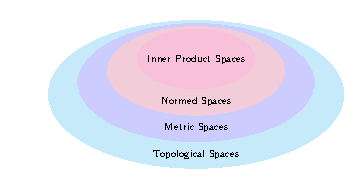
\includegraphics[scale=2]{doc/structure_spaces/structure_spaces.pdf}
	\caption{Overview of the generality of different spaces}
\end{figure}

\begin{theorem}{Pythagoral Theorem}{pyth_theo}
	Let $V$ be an Euclidean/Hermitian vector space and $u, v \in V$ with $u \perp v$. Then 
	\[
		\Vert u + v \Vert ^2 = \Vert u \Vert ^2 + \Vert v \Vert ^2.
	\]
\end{theorem}



